\section{Packet transactions}
\label{s:transactions}

\begin{figure*}[!t]
\begin{subfigure}{0.5\textwidth}
\begin{small}
\begin{lstlisting}[style=customc]
#define NUM_FLOWLETS    8000
#define THRESH          5
#define NUM_HOPS        10

struct Packet {
  int sport;
  int dport;
  int new_hop;
  int arrival;
  int next_hop;
  int id; // array index
};

int last_time [NUM_FLOWLETS] = {0};
int saved_hop [NUM_FLOWLETS] = {0};

void flowlet(struct Packet pkt) {
  pkt.new_hop = hash3(pkt.sport,
                      pkt.dport,
                      pkt.arrival)
                % NUM_HOPS;

  pkt.id  = hash2(pkt.sport,
                  pkt.dport)
            % NUM_FLOWLETS;

  if (pkt.arrival - last_time[pkt.id] @\label{line:ifStart}@
      > THRESH)
  { saved_hop[pkt.id] = pkt.new_hop; } @\label{line:ifEnd}@

  last_time[pkt.id] = pkt.arrival;
  pkt.next_hop = saved_hop[pkt.id];
}
\end{lstlisting}
\end{small}
\caption{Flowlet switching written in \pktlanguage}
\label{fig:flowlet_code}
\end{subfigure}
%
%
\begin{subfigure}{0.4\textwidth}
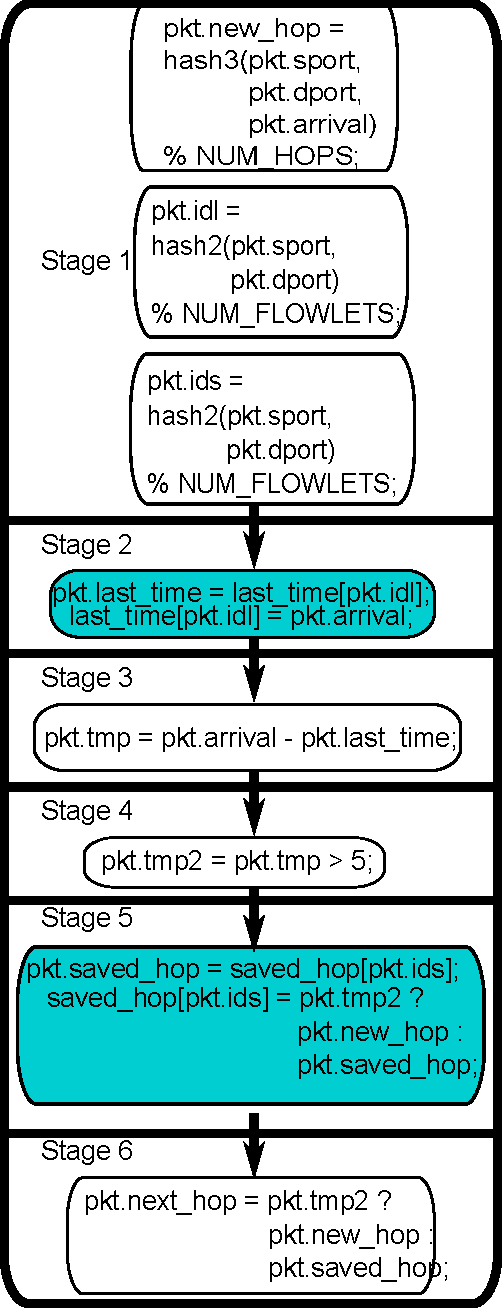
\includegraphics[width=0.9\columnwidth]{pipe.pdf}
\caption{6-stage \absmachine pipeline for flowlet
switching.  Control flows from top to bottom. Stateful atoms are in grey.}
\label{fig:flowlet_pipeline}
\end{subfigure}
\caption{Programming flowlet switching in \pktlanguage}
\end{figure*}

A programmer programs a data-plane algorithm by writing it as
a packet transaction in \pktlanguage (Figure~\ref{fig:flowlet_code}).  The
\pktlanguage compiler then compiles this transaction to an atom pipeline for a
\absmachine machine (Figure~\ref{fig:flowlet_pipeline}). We first describe
packet transactions in greater detail by walking through an example
(\S\ref{ss:flowlet}). Next, we discuss language constraints in \pktlanguage
(\S\ref{ss:constraints}) informed by line-rate switches.  We then discuss
triggering packet transactions (\S\ref{ss:guards}) and handling multiple
transactions (\S\ref{ss:multiple}).

\subsection{\pktlanguage by example}
\label{ss:flowlet}

We use flowlet switching~\cite{flowlets} as our running example. Flowlet
switching is a load-balancing algorithm that sends bursts of packets, called
flowlets, from a TCP flow on a randomly chosen next hop, provided the bursts
are separated by a large enough time interval to ensure packets do not arrive
out of order at a TCP receiver. For ease of exposition, we use only the source
and destination ports in the hash function that randomly computes the next hop
for flowlet switching.
%it is easy to extend it to the full 5-tuple.

Figure~\ref{fig:flowlet_code} shows flowlet switching in \pktlanguage and
demonstrates its core language constructs. All packet processing happens in the
context of a packet transaction (the function \texttt{flowlet} starting at line
17). The function's argument type {\tt Packet} declares the fields in a packet
(lines 5--12)\footnote{A field is either a packet header, e.g.,
source port ({\tt sport}) and destination port ({\tt dport}), or packet
 metadata ({\tt id}).} that can be referenced by the function body (lines
18--32).  The function body can also modify persistent switch state using
global variables (e.g., \texttt{last\_time} and \texttt{saved\_hop} on lines 14
and 15, respectively). The function body may use \textit{intrinsics} such as
\texttt{hash2} on line 23 to directly access hardware accelerators on the
switch such as hash generators.  The \pktlanguage compiler uses an intrinsic's
signature to analyze read/write dependencies (\S\ref{ss:pipelining}), but otherwise considers it a blackbox.

\medskip
\noindent
\textbf{Packet transaction semantics.}
Semantically, the programmer views the switch as invoking the packet transaction
serially in the order in which packets arrive, with no concurrent packet
processing.  Put differently, the packet transaction modifies the passed-in
packet argument and runs to completion, before starting on the next packet.
These semantics allow the programmer to program under the illusion that a
single, extremely fast, processor is serially executing the packet processing code for
all packets. The programmer doesn't worry about parallelizing the code within
and across pipeline stages to run at line rate.

\subsection{The \pktlanguage language}
\label{ss:constraints}
\pktlanguage's syntax (Figure~\ref{fig:grammar}) is similar to C, but with
several constraints (Table~\ref{tab:restrict}).  These constraints are required
for deterministic performance.  Memory allocation, unbounded iteration counts,
and unstructured control flow cause variable performance, which may prevent an
algorithm from achieving line rate. Additionally, within a \pktlanguage transaction, 
each array can only be accessed using a single packet field, and repeated accesses to the 
same array are allowed only if that packet field is unmodified between accesses.
%array modifications by mandating that a single execution of a transaction (the
%execution of a transaction for a single packet) can access only one entry in an
%array.

For example, all read and write accesses to \texttt{last\_time} use the
index \texttt{pkt.id}. \texttt{pkt.id} is not modified during the
course of a single transaction execution (single packet); it only changes between executions
(packets).  This restriction on arrays mirrors restrictions on the stateful memories
attached to atoms (\S\ref{s:atomConstraints}), which require multiple ports to
support distinct read and write addresses every clock cycle.

\begin{table}
  \begin{tabular}{p{0.95\columnwidth}}
   No iteration (while, for, do-while).\\
   No unstructured control flow (goto, break, continue).\\
   No heap, dynamic memory allocation, or pointers.\\
   At most one location in each array is accessed by a single execution of a transaction. \\
   No access to unparsed portions of the packet (payload).\\
  \end{tabular}
  \caption{Restrictions in \pktlanguage}
  \label{tab:restrict}
\end{table}

\begin{figure}
\newcommand{\sep}{~|~}
\begin{scriptsize}
\begin{eqnarray*}
l \in \text{literals} \quad v \in \text{variables} \quad &bop& \in \text{binary ops} \quad
uop \in \text{unary ops} \\
%
e \in \text{expressions} &::=& e.f \sep l \sep v \sep e~bop~e \sep uop~e \sep e[d.f] \sep \\
                   & &   f(e_1, e_2, \ldots) \\
%
s \in \text{statements} &::=& e = e \sep {\tt if}~(e)~\{ s \}~{\tt else}~ \{ s \} \sep s~;~s \\
%
t \in \text{packet txns} &::=& name(v) \{ s \} \\
%
%vlist \in varList &::=& var;vlist \sep vlist \\
%
d \in \text{packet decls} &::=& \{ v_1, v_2, \ldots \} \\
%
sv \in \text{state var inits} &::=& v = e \sep sv~;~sv \\
%
p \in \text{\pktlanguage programs} &::=& \{ d ; sv; t \}
\end{eqnarray*}
\end{scriptsize}
\caption{\pktlanguage grammar. Type annotations (void, struct, and int) are elided for simplicity.}
\label{fig:grammar}
\end{figure}


\subsection{Triggering packet transactions}
\label{ss:guards}
Packet transactions specify \textit{how} to process packet headers and state.  To
specify {\em when} to run packet transactions, programmers use {\em guards}:
predicates on packet fields that trigger a transaction if a packet
matches the guard. For example, {\tt (pkt.tcp\_dst\_port == 80)} would
trigger heavy-hitter detection~\cite{opensketch} on packets with TCP
destination port 80.

Guards can be realized using an exact match in a match-action table, with the
actions being the atoms compiled from a packet transaction. Guards
can take various forms, e.g., exact, ternary, longest-prefix, and range-based
matches, depending on the matches supported by the match-action
pipeline. Because guards map straightforwardly to the match key in a
match-action table, we focus only on compiling packet transactions in this paper.

\subsection{Handling multiple transactions}
\label{ss:multiple}
So far, we have discussed a single packet transaction corresponding to a single
data-plane algorithm. In practice, a switch would run multiple data-plane
algorithms, each processing its own subset of packets. To address this, we
envision a policy language that specifies pairs of guards and transactions.
Realizing a policy is straightforward when all guards are disjoint. When guards
overlap, multiple transactions need to execute on the same subset of packets,
requiring a mechanism to compose transactions.

One composition semantics is to run the two transactions one after another
sequentially in a user-specified order. This can be achieved by concatenating
the two transaction bodies to create a larger transaction.  We leave a detailed
exploration of multiple transactions to future work, and focus only on
compiling a single packet transaction here.
